\section{Introduction}
\label{s:introduction}

%% \begin{outline}

%%   \textbf{Page budget: 2-2.5 pages. Longer intro.}

%%   Today's 2D infrastructure: summarize how on-demand and live works today. Make the point that live is compressed and streamed when content is generated, and on-demand is compressed and stored (maybe also talk about decoupled content creation and compression in YouTube). We expect that 3D infrastructure will follow a similar architecture.

%%   We focus on dynamic 3DGS content distribution:
%%   \begin{itemize}
%%   \item Briefly explain what dynamic 3DGS (henceforth \dgs{}, the 4th dimension being time) 
%%   \item Describe how it is represented: per-frame Gaussians with attributes
%%   \item How each frame is produced: trained from multi-camera image sequences
%%   \end{itemize}

%%   \begin{itemize}
%%   \item Why 4DGS is interesting: free-viewpoint, higher quality than point clouds, less weighty than meshes. (Make other points as necessary).
%%   \item Why it is challenging: extremely large, even single-participant scenes require large amounts of data; infeasible to stream, especially to mobile devices
%%   \end{itemize}

%%   Thus, to come within the realm of feasibility, must be able to compress 4DGS. We consider compression for streaming. Goal of compression for streaming: reduce information to fit within a given target bitrate.

%%   Two approaches:
%%   \begin{description}
%%   \item[During-Training Compression] Reducing the number of Gaussians, transforming attributes to a neural feature space, residual representations for inter-frame compression: (*) means we compare against
%%     \begin{itemize}
%%     \item Reducing Gaussians: QUEEN(*) and V3(*)
%%     \item Transforming attributes Vega
%%     \item Inter-frame compression: QUEEN(*)
%%     \end{itemize}
%%   \item[Post-Training Compression] By itself, during-training compression can be augmented to fit within bandwidth targets (e.g., by incorporating a quantizer and the target during training). Recent work has considered an alternative approach: post-training compression, which takes as input 3DGS frames and encodes their attributes by extending existing point-cloud or 2D codecs. This can compress 4DGS to a given bitrate, for example, by adjusting quantization levels. 
%%     \begin{itemize}
%%     \item 2D codecs: V3(*)
%%     \item Unmodified point cloud: G-PCC based (Haoran's (*))
%%     \item Modified/Adapted: LTS(*), Meson GS
%%     \end{itemize}
%%   \end{description}

%%   Our focus is on post-training compression. Post-training compression can be more compute-efficient and flexible. Flexible because it can encode at bitrates not envisaged during training. Efficient because (like post-training model quantization) it can avoid training costs. \ramesh{Raj, send me numbers for overhead of in-training quantizers.}

%%   Our goal is to develop a compute-efficient real-time codec for 4DGS post-training compression, especially one that takes a step towards real-time decoding on a mobile device. None of the existing methods can encode and decode in real-time (V3 can decode in realtime): Add per-frame encode and decode times for V3/MesonGS/LTS/GPCC and \gsnfs{}.
  
%%   Efficient decoding is useful, but why is efficient encoding useful?
%%   \begin{itemize}
%%   \item Can reduce compute cost for encoding \dgs{} videos (add a table of costs per frame for V3/MesonGS/LTS/GPCC and \gsnfs{} for a 1-hour video), especially since we may need to encode at different bitrates.
%%   \item In the future, emerging feed-forward \dgs{} networks can generate at frame rate (GPS-Gaussian), may be able to live-stream, need 30 fps for this.
%%   \end{itemize}

%%   Approach: Following recent work, we extend point-cloud compression techniques to \dgs{}. These encode geometry and attributes separately, contain methods to trade-off quality using quantization, and perform entropy coding. Prior work uses Draco/G-PCC, and times shown in the table.

%%   Although we use an identical architecture, we must be able to reduce encode/decode times to less than 30 ms per frame, 1--2 orders of magnitude less than current approaches. Clearly, to achieve this we must employ fine-grain parallelism.

%%   Challenges:
%%   \begin{itemize}
%%   \item Many different choices of components (octree vs k-d tree for position encoding), attribute transforms (hierarchical vs. Predictive transform coding), standard entropy coding vs arithmetic coding. What set of architecture components permits parallel implementation? \ramesh{Think about right way to say this; perhaps say plausibly parallelizable.}
%%   \item How exactly can these components be efficiently parallelized? None of these components are actually known to be parallelizable.
%%   \item Can we exploit this parallelism to improve compressibility \textit{and} quality?
%%   \end{itemize}

%%   \ramesh{Depending on results, we may need to contextualize results against V3 by comparing VPCC and GPCC.}

%%   Contributions:
%%   \begin{itemize}
%%     \item Octree decomposition, hierarchical transforms and a lossless entropy encoder.
%%     \item Highly parallel, GPU implementation, for encoding/decoding based on key algorithmic insight: using the Morton code as the backbone for enabling parallelism because of the observation that Morton code can be used to cheaply determine parents and children, so we have a new paradigm for parallelism (parallel at each level of octree, logarithmic iterations). This enables both octree and RAHT.
%%   \item Novel optimal color de-correlation exploiting GPU parallelism, selective attribute quantization based on fast search of quality spaces
%%   \end{itemize}

%%   Results: present all the results and make special mention of the 2D codec comparisons as well.

%%   Make the point that a lot of our work applies to point clouds as well and enables fast point-cloud compression (maybe even add a simple experiment on Panoptic data?).
  
%% \end{outline}

Video over the Internet has effected societal and economic transformations.
%
A technology with potentially similar transformative power, 3D video, is on the horizon.
%
In 3D video, each frame depicts a representation of a scene in three dimensions, and viewers can view the scene from any perspective.
%
This technology will enable entirely new ways of viewing sporting events, and new modes of instruction delivery, as well as new visual story-telling paradigms.

\subsection{Gaussian Splatting}\label{sec:3d-gauss-splatt}

%\parab{Background.}
%
At the core of any 3D video technology is a technique to represent a 3-D scene.
%
While many representations exist, 3-D Gaussian Splats~\cite{kerbl3Dgaussians} (or \gs{}) have been the subject of recent research interest.
%
\gs{} represents a scene as a collection of 3-D Gaussians.
%
Each Gaussian represents a small, ellipsoidal volume, and is defined by its position in 3-D and a set of attributes.
%
The Gaussians and their attributes are learned by training on a set of camera images capturing a scene from multiple perspectives.
%
For this reason, we refer to the set of Gaussians and their attributes as a \gs{} model.

More precisely, a \gs{} model is a collection of $N$ 3D Gaussians, each with the following \textit{attributes}:
\begin{itemize}
\item Mean ($\in \mathbb{R}^3$) represents the position of the Gaussian in 3D space (\textit{i.e.}, the center of the ellipsoid).
\item Scales ($\in \mathbb{R}^3$) define the size of the ellipsoid along its three axes.
\item Rotation ($ \in \mathbb{R}^4$) defines the orientation of the ellipsoid in 3D space, typically represented as a quaternion.
\item Opacity ($ \in \mathbb{R}$) represents the transparency of the Gaussian.
\item Colors: In \gs{}, spherical harmonics (SH), which are functions defined on a surface, represent view-dependent color, capturing realistic lighting effects, material properties, and reflections.
%
Each SH function is represented by three coefficients corresponding to three colors (RGB).  
%
The coefficients of a degree $d = 0$ SH---the DC coefficients---represent the overall color of the Gaussian.
%
Higher degree ($d > 0$) AC coefficients capture more complex lighting and shading effects.
%
A common choice of SH degree is 3, which results in $48$ SH coefficients per Gaussian.%\eduardo{16 for each color channel}
\end{itemize}
%
Given a \gs{} model and a viewpoint, a rendering algorithm~\cite{kerbl3Dgaussians} produces an image of the view of the scene from the given perspective.
%
While training a \gs{} model can take minutes, rendering only requires milliseconds.

\begin{figure*}[t]
  \centering
  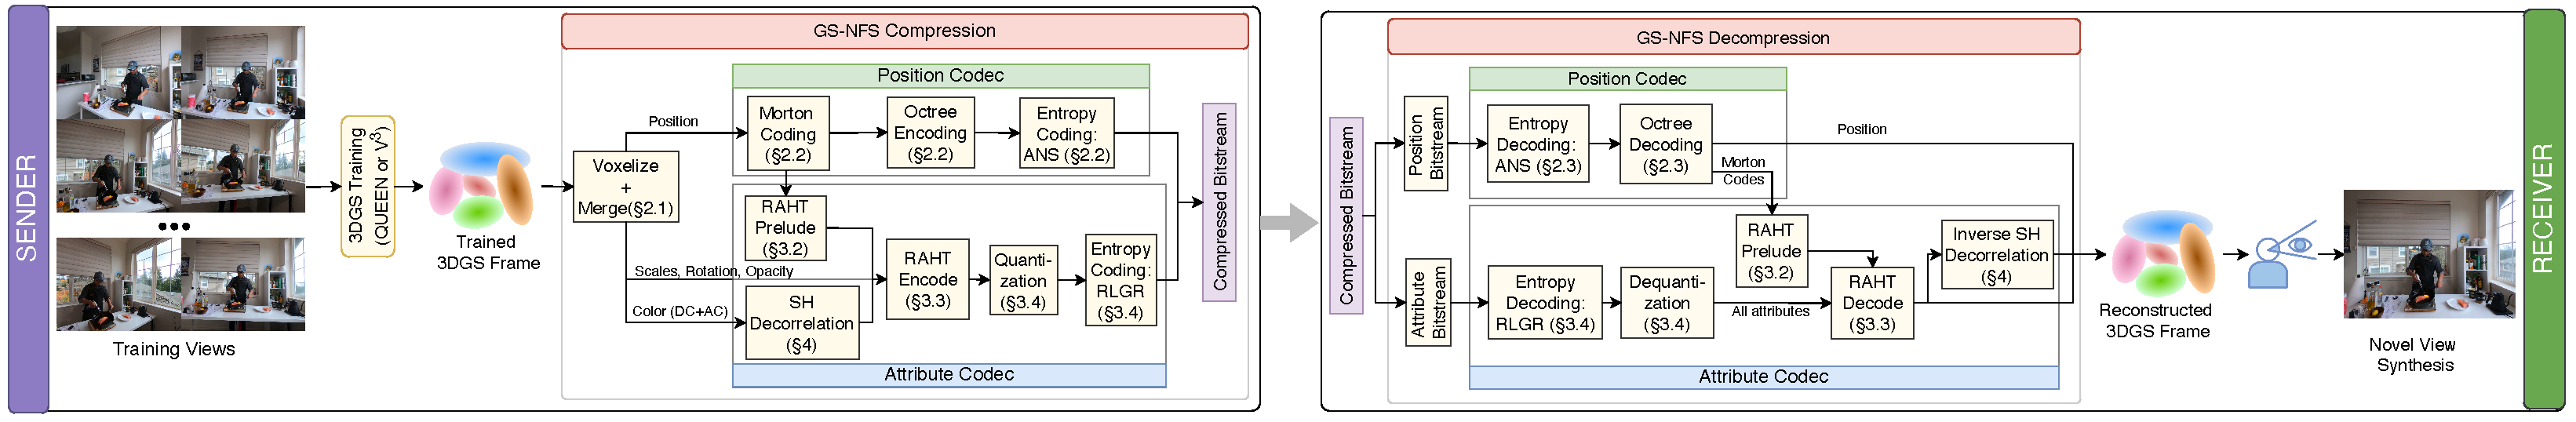
\includegraphics[width=\textwidth]{figures/architecture.pdf}
  \caption{\gsnfs Architecture. Blocks in yellow are GPU-resident components.}
  \label{fig:architecture}
\end{figure*}

\parab{Dynamic \gs{}.}
%
A sequence of \gs{} frames constitutes a \textit{dynamic} \gs{} video, often referred to as \dgs{} (time being the fourth dimension).
%
In this paper, we focus on delivery of \dgs{} content.
%
This delivery is challenging, because each \gs{} frame can be large.
%
Each Gaussian requires about 236 bytes to represent its attributes.
%
\gs{} frames with a million Gaussians are not uncommon, so a single frame can be 236~MB in size.
%
By contrast, a single frame of 4K UHD video requires 24-30~MB, an order of magnitude less.

\subsection{\dgs{} Compression}\label{sec:dgs-compression}

To reduce the size of \dgs{}, recent work has explored compression techniques.
%
In addition to reducing size, compression can be used to encode \dgs{} at different bitrate levels for streaming, as for 2D video.
%
Two \textit{complementary} approaches have emerged (\cref{sec:related-work} discusses related work in detail).

\textit{During-training} compression techniques reduce information in a variety of ways.
%
%For example, 
QUEEN~\cite{queen}, 4DGC-Pro~\cite{zheng20254dgcproefficienthierarchical4d}, and CompGS++~\cite{compgsplus} reduce the number of Gaussians by using temporal prediction between key frames and their immediately following frames.
%% \ao{Grouping is confusing. It seems to refer to something similar to GOPs (groups of pictures) in video coding, but the gain does not come from grouping; it comes from motion estimation and compensation. In this case, if residuals are generated, it sounds like current Gaussians are predicted from past Gaussians and this sounds more like "temporal prediction", rather than grouping. }
%
A frame following a key frame is represented using \textit{residuals}---differences with respect to the key frame.
%
Other approaches exploit human tolerance for small color distortions.
%
Vega~\cite{Vega} compresses SH (color) coefficients aggressively by first grouping semantically-related Gaussians, then training an MLP for each Gaussian group.
%
QUEEN~\cite{queen} and 4DGC-Pro~\cite{zheng20254dgcproefficienthierarchical4d}  also train a quantizer that can learn optimal quantization levels for SH coefficients. %\ramesh{Add some text after Raj gives numbers for during-training quantization.}
%
Quantization reduces the number of bits required to represent SH coefficients at the expense of information loss.

\textit{Post-training compression} techniques take a sequence of \gs{} frames as input and encode Gaussian attributes using 2-D or 3-D video codecs.
%
For example, \vthree{}~\cite{v3volumetric} encodes Gaussian attributes in images and compresses the image sequence using a H.264 codec.
%
MesonGS~\cite{mesongs} and LTS~\cite{LTS} extend point-cloud compression techniques, such as G-PCC~\cite{gpcc} or Draco~\cite{draco}, to compress \dgs{}.
%
Post-training compression has two advantages: (a) it can be faster than during-training compression (\cite{queen} reports about a 20\% increase in training time with a during-training quantizer), and (b) it can help encode \dgs{} videos at different bitrates without re-training.



\subsection{Approach, Challenges, and Contributions}\label{sec:appr-chall-contr}

\parab{Goal.}
%
We present \gsnfs{} (or GS-NFS)\footnote{NFS, or Need for Speed, is a popular car racing game.}, a post-training compression method for \dgs{} which can encode and decode at full frame-rate, 30 frames per second (fps).
%
It is also mobile-friendly; on a mobile GPU, it can decode some \dgs{} sequences at 25~fps.
%
No prior work on post-training compression has achieved full frame rate encode and decode.

% % DO NOT use LaTeX markup for header line of csv
% \begin{filecontents}[overwrite,noheader]{encode-decode-intro.csv}
% Time;VideoGS;MesonGS;LTS;G-PCC;GSStream
% \textbf{Encode};;;;;
% \textbf{Decode};;;;;
% \end{filecontents}

% \begin{table}[t]
%   \scalebox{0.8}{
% \csvreader[%
% tabular = |l|c|c|c|c|c|,%
% table head = \hline \textbf{Time (ms)} & \textbf{VideoGS} & \textbf{MesonGS} & \textbf{LTS} & \textbf{G-PCC} & \textbf{\gsnfs{}} \\ \hline\hline,%
% separator = semicolon,%
% late after line = \\ \hline%
% ]{encode-decode-intro.csv}{}{\csvlinetotablerow}}
%   \caption{Encode and decode times for \gsnfs{} and competing approaches for a frame from a sequence in the Neural3D dataset.}
%   \label{tab:encode-decode}
% \end{table}

Full frame-rate decoding is obviously useful; without that, it will not be possible to play \dgs{} videos at frame rate.
%
We argue that full frame-rate \textit{encoding} is useful for 
% it said two previously 
three important reasons.
%
First, for on-demand streaming, it will be necessary to encode \dgs{} videos at different bitrates.
%
At scale, an efficient encoder can reduce dollar costs significantly for encoding in the cloud.
%
%% \cref{tab:encode-cost} shows the cost of encoding an hour-long \dgs{} video sequence; \gsnfs{} is at least an order of magnitude cheaper than other approaches.
%
Second, today, 2D video providers use per-title \textit{encode optimization}~\cite{netflix_rdo}.
%
This approach seeks to find the best quality to encode a video, by repeatedly encoding and decoding frames at different qualities.
%
A fast encoder/decoder like \gsnfs{}'s can enable similar optimizations for \dgs{}.
%
Third, recent work in feed-forward \gs{} networks~\cite{zhou2024gpsplus} can generate Gaussian frames within tens of milliseconds.
%
This can generate Gaussian frames at nearly full frame rate, and \gsnfs{} can help encode and transmit these frames in real-time.
%% \ao{Do we want to mention AI systems that use world models based on GS for training? In this scenario, having fast decoding enables reduction of memory bandwidth with near lossless representation and low latency. } 

% DO NOT use LaTeX markup for header line of csv
%% \begin{filecontents}[overwrite,noheader]{encode-costs.csv}
%% ;VideoGS;MesonGS;LTS;GPCC;GSStream
%% \textbf{Encode Cost};;;;;
%% \end{filecontents}

%% \begin{table}[t]
%%   \scalebox{0.8}{
%% \csvreader[%
%% tabular = |l|c|c|c|c|c|,%
%% table head = \hline & \textbf{VideoGS} & \textbf{MesonGS} & \textbf{LTS} & \textbf{GPCC} & \textbf{\gsnfs{}} \\ \hline\hline,%
%% separator = semicolon,%
%% late after line = \\ \hline%
%% ]{encode-costs.csv}{}{\csvlinetotablerow}}
%%   \caption{Estimated cloud encode costs for an hour-long \dgs{} full-scene video such as the ones in the Neural3D dataset. We estimated these by measuring encode times for each approach, then obtaining the cost for the corresponding machine configurations from a cloud provider.}
%%   \label{tab:encode-cost}
%% \end{table}

\parab{Approach.}
%
To achieve this goal, \gsnfs{} uses a compression approach similar to a point-cloud compression technique, G-PCC~\cite{gpcc}.
%
This is a more natural starting point than the 2D compression used in \vthree{}~\cite{v3volumetric}, since a \gs{} frame's representation resembles that of a point-cloud.
%
The latter contains a set of points, each with one or more attributes; \gs{} is similar, except that each Gaussian has more attributes (\cref{sec:3d-gauss-splatt}).
%
Next, we describe the G-PCC pipeline for encoding \gs{} frames; MesonGS~\cite{mesongs} has used such an approach.

G-PCC~\cite{gpcc}'s encoder takes a set of positions and associated attributes as input, then serializes (produces a bitstream) this set for transmission.
%
Its decoder reconstructs the positions and attributes from the bitstream.
%
To do this, G-PCC (a) \textit{encodes} positions and associated attributes in such a manner that they can be decoded efficiently, and (b) compresses these encodings (either with or without information loss) to ensure bandwidth and storage efficiency.

G-PCC encodes position and attributes using qualitatively different approaches.
%
It represents positions of Gaussians using a spatial data structure, an \textit{octree}.
%
Usually, \gs{} Gaussians are spatially sparse, so not all parts of the octree are occupied.
%
G-PCC serializes the octree such that the bitstream only contains information for occupied octree parts.

For attributes, G-PCC provides several alternatives.
%
We use Region-Adaptive Hierarchical Transform (RAHT~\cite{raht,de2016compression}), which organizes the Gaussians into a hierarchy of levels and predicts attributes at finer levels from attributes at coarser levels.
%
The output of RAHT is a set of coefficients, which can be \textit{quantized} (this introduces loss) and then entropy-coded (a lossless step that removes redundancy).

G-PCC's decode pipeline inverts these operations, de-serializing Gaussians from the encoded bitstream.
%
Unfortunately, G-PCC and MesonGS have high encode and decode times (\cref{sec:baseline-comparisons}).
%
\gsnfs{} achieves frame-rate encode/decode by \textbf{\textit{running the entire encoding and decoding pipeline on a GPU}}.
%
Beyond accelerating encoding, executing the encoder on a GPU is efficient when the encoder takes input from a training method that emits \gs{} frames.
%
These frames are already in GPU memory, since \gs{} training requires a GPU, thereby avoiding memory copy costs.

\parab{Challenges and Contributions.}
%
Unfortunately, accelerating G-PCC's algorithms on a GPU is non-trivial.
%
Unlike 2D video frames, where pixels exhibit regularity, \gs{} training can produce irregularly-spaced Gaussians.
%
Mapping this to a single-instruction, multi-threaded (SIMT) GPU is difficult.

CPU-resident algorithms for octree encoding and RAHT manage this irregularity by imposing a spatial hierarchy on the data.
%
Unfortunately, GPUs are a poor fit for computations on hierarchical data.
%
Traversing the hierarchy requires following pointers; this \textit{pointer chasing} is known to be highly inefficient on a GPU, since if the referenced memory is not in the cache, all warps in a GPU thread must wait for the data to be loaded (sometimes from relatively slow DRAM), resulting in poor performance.
%
This problem is well-known for GPU-based computations on irregular data in general~\cite{pointer_chasing1,pointer_chasing2}, and for parallelizing point-cloud algorithms in particular~\cite{groot,octree-gpu2011}.

Against this backdrop, \gsnfs{} is, to our knowledge, the first post-compression encoder/decoder for \dgs{} in which \textit{all} components (\cref{fig:architecture}) execute on a GPU and can encode and decode at full frame rate.
%
To achieve this, the paper makes the following novel contributions:
\begin{itemize}
\item A GPU-based parallelization of octree encoding (\cref{sec:gpu-octree}).
\item A GPU-based parallelization of RAHT (\cref{sec:gpu-raht}).
\item A technique to improve the compression of \dgs{} (\cref{sec:klt}). \end{itemize}

Our evaluations (\cref{sec:evaluation}) on two different popular \dgs{} datasets demonstrate that \gsnfs{}: (a) can encode an order of magnitude faster than the state-of-the-art; (b) dominates MesonGS~\cite{mesongs}, a GPCC~\cite{gpcc-adaptive} variant modified for \dgs{}, and LTS~\cite{LTS} both in quality and compression performance, and performs comparably or better than \vthree{}~\cite{v3volumetric} on large scenes; (c) can decode \dgs{} at up to 25~fps on a Jetson Orin; and (d) can encode and decode point clouds and live \dgs{} videos at full frame rate, a capability that, to our knowledge, has not been demonstrated in the literature.

%% \begin{outline}

%%   \textbf{Page budget: 2-2.5 pages. Longer intro.}

%%   Today's 2D infrastructure: summarize how on-demand and live works today. Make the point that live is compressed and streamed when content is generated, and on-demand is compressed and stored (maybe also talk about decoupled content creation and compression in YouTube). We expect that 3D infrastructure will follow a similar architecture.

%%   We focus on dynamic 4DGS content distribution: higher quality than point clouds, less weighty than meshes. (Make other points as necessary).
  
%%   Problem setup:
%%   \begin{itemize}
%%   \item Why GS compression is important
%%   \item Why is bandwidth-adaptivity important (make the point that bandwidth-adaptive means making principled quality-compression tradeoffs, unlike encoding 3D in 2D) \eduardo{You can still do bandwidth adaptivity by encoding in 2D. The method you described in our last meeting can do it because it is based on a video codec.  It may be too complex, or suboptimal, etc., but still possible.}
%%   \item What are the different approaches: in-training and post-training?
%%   \end{itemize}
  

%%   Briefly cover related work:
%%   \begin{description}
%%   \item[During-Training Compression] Reducing the number of Gaussians, transforming attributes to a neural feature space, residual representations for inter-frame compression (*) means we compare against
%%     \begin{itemize}
%%     \item Reducing Gaussians: QUEEN(*) and V3(*)
%%     \item Transforming attributes Vega
%%     \item Inter-frame compression: QUEEN(*)
%%     \end{itemize}
%%   \item[Post-Training Compression] Usually leverages existing point-cloud or 2D codecs or variations thereof
%%     \begin{itemize}
%%     \item 2D codecs: V3(*)
%%     \item Unmodified point cloud: G-PCC based (Haoran's (*))
%%     \item Modified/Adapted: LTS(*), Meson GS
%%     \end{itemize}
%%   \end{description}
%%   Of these, only Haoran's work is bandwidth-adaptive. Make a table of closely related work and show how we occupy a unique point in the design space (figure out what the dimensions are).

%%   Our focus: 30fps post-training, bandwidth-adaptive, compression and decompression of 4DGS data (somewhere mobile-friendly should show up)

%%   Why 30fps:
%%   \begin{itemize}
%%   \item Today's mature 3D codecs are extremely slow for encoding and decoding: add table for G-PCC and Draco for point cloud
%%   \item Achieving higher frame rates can help on-demand 3D videos to reduce the compute cost of encoding
%%   \item Emerging feed-forward 4DGS networks can generate at frame rate (GPS-Gaussian), may be able to live-stream, need 30 fps for this.
%%   \end{itemize}

%%   Why compression and bandwidth-adaptive: use arguments from LiVO paper.

%% \eduardo{You might want to discuss our goals before you talk about during-training and post-training. Then discuss during-training with respect to those goals. Then discuss post-training with respect to those goals. Then explain our choices.}
%%   Why post-training:
%%   \begin{itemize}
%%   \item Decoupling of training from compression is helpful for different bitrate combinations (wired/wireless, different clients); for 4DGS, much more complicated to do this
%%   \item Enables live (feed-forward networks may or not be able to compress live, we don't know of any now). \ramesh{Raj, please check this.}
%%   \item Does not eliminate the need for during-training compression; these are complementary (as we discuss later).
%%   \end{itemize}

%%   Post-training compression primer: most papers encode 4DGS data by extending point cloud compression techniques. There are two mature ones: Draco and G-PCC. Similar architecture: geometry encoding, attributed encoding, entropy coding. Both are intra-frame only.

%%   Table with breakdown of current encode and decode times of Draco/G-PCC components for ActorsHQ data. Table can include the specific algorithms used for each piece. Add also compression factors to make the point that choice of algorithms can result in different tradeoffs of compression and run-time. (We do this to make the point that we use the same architecture, but find a different point in the compressibility/run-time trade-off space). All of these numbers are on CPUs.

%%   %% GPU pipeline, r-d curves, decorrelation in part of attribute space

%%   Challenges:
%%   \begin{itemize}
%%   \item How to enable post-training compression at 30 fps (especially given the numbers in the table)? (Point out that we would sacrifice compressibility). \eduardo{You can say, simple architecture, where each component is parallelizable. And other codecs are a lot more complicated, and have non-parallelizable components?}
%%   \item How to achieve high-quality, while enabling bandwidth-adaptivity?
%%   \end{itemize}

%%   Contributions:
%%   \begin{itemize}
%%   \item Highly parallel, GPU implementation, for encoding/decoding based on key algorithmic insight: using the Morton code as the backbone for enabling parallelism because of the observation that Morton code can be used to cheaply determine parents and children, so we have a new paradigm for parallelism (parallel at each level of octree, logarithmic iterations). This enables both octree and RAHT.
%%   \item High-quality bandwidth-adaptive, which adaptively quantizes different attributes of 3D Gaussians based on human sensitivity to geometry and color. Adaptive quantization enabled by novel decorrelation.
%%   \end{itemize}

%%   Results: present all the results and make special mention of the 2D codec comparisons as well.

%%   Make the point that a lot of our work applies to point clouds as well and enables fast point-cloud compression (maybe even add a simple experiment on Panoptic data?).
  
%% \end{outline}

